%
% main.tex
%
% This file contains only the skeleton of the technical note:
%  * package import and setup
%  * page setting
%  * author list
%  * title page
% 
% The rest of the content is imported from other files.
%


\documentclass{article}

% \usepackage[margin=1in]{geometry} 
\usepackage{amsmath,amsthm,amssymb,amsfonts}
\usepackage{float}
\usepackage{graphicx}
\usepackage{fancyhdr}
% \usepackage{url}           % for on-line citations
% \usepackage{bm}            % special 'bold-math' package 
% \usepackage{graphics}      % standard graphics specifications
\usepackage{authblk}  % allows more complex multi-author, multi-affiliation author list
\usepackage{natbib}   % bibliography as Overleaf likes

% \usepackage[dvipsnames,table]{xcolor}
% \usepackage{subfig}


%for the links
% \usepackage{color}
\usepackage{hyperref}
\hypersetup{
    colorlinks=true, % make the links colored
    linkcolor=blue, % color TOC links in blue
    urlcolor=red, % color URLs in red
    linktoc=all
    } % 'all' will create links for everything in the TOC

\usepackage{cleveref} % \cref and \Cref for "clever" reference text; needs to be loaded after hyperref

% \usepackage{sectsty}
% \subsectionfont{\fontsize{12}{15}\selectfont\centering}
% \sectionfont{\fontsize{12}{15}\selectfont\centering}
% \renewcommand\thesection{\Roman{section}}
% \renewcommand\thesubsection{\Alph{subsection}}
% \renewcommand{\familydefault}{\updefault}

% Set up fancy header/footer
\pagestyle{fancy}
\fancyhead[LO,L]{}
\fancyhead[CO,C]{\title{}}
\fancyhead[RO,R]{}
\fancyfoot[LO,L]{}
\fancyfoot[CO,C]{\thepage}
\fancyfoot[RO,R]{}
% \renewcommand{\headrulewidth}{0.4pt}
% \renewcommand{\footrulewidth}{0.4pt}

\providecommand{\tightlist}{%
  \setlength{\itemsep}{0pt}\setlength{\parskip}{0pt}}

%%%%%%%%%%%%%%%%%%%%%%%%%%%%%%%%%%%%%%%%%%%%%%%%%%%%%%%%%%%%%%%%%%%%%%%%%%%%%%%%
%%% Macro definitions
%%%

%
% LaTeX definitions for this note
%
% Requires: xspace
%

\usepackage{xspace}
\usepackage{upgreek}  % \upmu...


% - - - - - - - - - - - - - - - - - - - - - - - - - - - - - - - - - - - - - - -
% physics quantities
% 
\newcommand{\micros}[1]{\ensuremath{#1}\,\ensuremath{\upmu{}}s}
\newcommand{\Hz}[1]{\ensuremath{#1}\,Hz}
\newcommand{\V}[1]{\ensuremath{#1}\,V}
\newcommand{\milliV}[1]{\ensuremath{#1}\,mV}
\newcommand{\kiloV}[1]{\ensuremath{#1}\,kV}
\newcommand{\nanoF}[1]{\ensuremath{#1}\,nF}
\newcommand{\mebiB}[1]{\ensuremath{#1}\,MiB}
\newcommand{\mm}[1]{\ensuremath{#1}\,mm}
\newcommand{\cm}[1]{\ensuremath{#1}\,cm}



% - - - - - - - - - - - - - - - - - - - - - - - - - - - - - - - - - - - - - - -
% ICARUS jargon
%
\newcommand{\DBB}{DBB\xspace}
\newcommand{\TPC}{TPC\xspace}
\newcommand{\ICARUSmodule}{T300\xspace}

\newcommand{\Chimney}[1]{\texttt{#1}}
\newcommand{\Cable}[1]{\texttt{#1}}


% - - - - - - - - - - - - - - - - - - - - - - - - - - - - - - - - - - - - - - -
% language

\newcommand{\eg}{e.g.\ }

% - - - - - - - - - - - - - - - - - - - - - - - - - - - - - - - - - - - - - - -



%%%%%%%%%%%%%%%%%%%%%%%%%%%%%%%%%%%%%%%%%%%%%%%%%%%%%%%%%%%%%%%%%%%%%%%%%%%%%%%%
%%% Front page definition
%%%


\title{ICARUS connectivity test --- December 2018}


\author[a]{Angela~Fava \thanks{afava@fnal.gov}}
\affil[a]{Fermi National Accelerator Laboratory}

\author[b]{Mark~Convery \thanks{convery@slac.stanford.edu}}
\author[b]{Gianluca~Petrillo \thanks{petrillo@slac.stanford.edu}}
\author[b]{Yun-Tse~Tsai \thanks{yuntse@slac.stanford.edu}}
\affil[b]{SLAC National Accelerator Laboratory}

\author[z]{Somebody~else \thanks{somebody@institution.edu}}
\author[z]{adding the others is a to-do \thanks{of course}}
\affil[z]{Someone's institution}

\date{\today}

%%%%%%%%%%%%%%%%%%%%%%%%%%%%%%%%%%%%%%%%%%%%%%%%%%%%%%%%%%%%%%%%%%%%%%%%%%%%%%%%
\begin{document}

\maketitle

\label{abstract}

\begin{abstract}
  We present here the procedure and results of the connectivity tests done on the TPCs wire planes of the ICARUS detector.
  All three, In\-duc\-tion-1, In\-duc\-tion-2 and Collection planes were tested.
  A test pulse was injected to each wire and an output signal was obtained and measured.
  An off-site analysis of the output signal waveforms was carried out for all standard and non-standard chimneys.
  As a result of the tests, we present a detailed description and mapping of how the detector is done from inside.
\end{abstract}



\tableofcontents

\section{Introduction}
\label{sec:Introduction}


Here goes an introduction to the document with a description of the structure and the content of each section. This may be the last part to be written, i.e. after all sections are completed.



\section{T600 Detector -- TPC (Time Projection Chamber)}
\label{sec:Detector}

detector done from inside.....


%To tests all the $53258$ wires that make up the whole ICARUS TPC without actually going inside the detectors it was decided to pull the connectors outside from the cryostat flanges through all the chimneys, to carefully and methodically inject a test pulse to the pulser cables that are directly connected to a board at the bottom of the vessel. To the same board is connected a single flat ribbon of 32-twisted cables connector that corresponds to only 32 wires of the TPC (Fig.). On top of the wire plane there's another board connected to another flat ribbon of those same 32 wires. This is the connector that then goes plugged-in to a test box. 



\section{Test methodology}
\label{sec:methodology}

This test follows broadly the same principles as the one performed in September
2018.
To test the electrical continuity, a test pulse is send, and a response is read,
this time from the connectors to the readout on the flange.
\\
We perform two tests, by probing two different paths.
The first path is equivalent to the one used in September 2018
(\cref{fig:PulseCables}): a test pulse is
sent through the test pulse cables at the bottom of the anode frame, where it is
distributed typically to 32 or 256 wires (for the single termination card and
for the eight daisy chained ones, respectively).
The pulse propagates through the wires, the termination card at the top of the
anode frame, the 68 pin cables, the \DBB and finally though the interface
connector on the flange, where it is picked up by our test apparatus.
The signal path within the \DBB (\cref{fig:WireToReadout}) can be appreciated
from \cite{ICARUSDBB}, where it enters through a ``WIRE'' port
(\eg \texttt{WIRE 16\_L}) and through the
\nanoF{10} capacitor induces onto the front end (\eg \texttt{FE 16\_L}).
\\
\begin{figure}
  \subfloat[test capacitance test]{
    \label{fig:WireToReadout}
    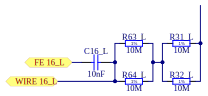
\includegraphics[width=0.48\textwidth]{fig/DBB-wire}
  }
  \subfloat[bias voltage test]{
    \label{fig:BiasVoltageToReadout}
    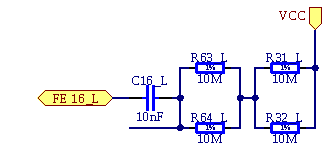
\includegraphics[width=0.48\textwidth]{fig/DBB-wire-HV}
  }
  \caption{
    DBB circuitry\cite{ICARUSDBB} involved in \protect\subref{fig:WireToReadout}
    test capacitance pulsing and \protect\subref{fig:BiasVoltageToReadout} bias
    voltage pulsing tests. The test pulse is entering through
    \protect\subref{fig:WireToReadout} ``WIRE'' and
    \protect\subref{fig:BiasVoltageToReadout} ``VCC'' port, and it is in both
    cases read out of the front-end port ``FE''.
    \label{fig:DBBcircuitryTest}
  }
\end{figure}
The second path (\cref{fig:BiasVoltageTestPath}) starts by pulsing a bias
voltage inlet.
\begin{figure}
  {
    \centering
    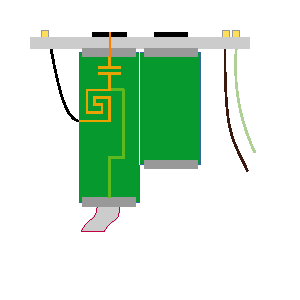
\includegraphics[height=6cm,clip,trim=0 30 0 0]{fig/BiasVoltagePath}\\
  }
  \caption{\label{fig:BiasVoltageTestPath}
    Illustration of the path of the test signal in the bias voltage connectivity
    test. The test pulse is injected through the bias voltage connector (left side),
    and follows a short path to the flange connector (represented in orange),
    bypassing the TPC wire (gray ribbon cable).
  }
\end{figure}
From there, the pulse is propagated to one side of the nine \DBB (labeled
``Cable AWG20'' in \cite{ICARUSDBB}) through the common and the channel-specific
circuitry (\cref{fig:BiasVoltageToReadout}) before reaching the front-end
readout.
It should be noted that the bias voltage circuitry is designed for a constant,
large voltage (\V{300}), while the test pulse is small (a few volt) and rapidly
changing.
Therefore, features observed in this test may be not significant for the regular
operation of the detector.
\\
These two paths test different paths of the circuitry
(\cref{fig:DBBcircuitryTest}).
The first path (\cref{fig:WireToReadout}), pulsing the wire through the test
capacitance, tests the full signal path, and barely grazes the \DBB circuitry.
The second one (\cref{fig:BiasVoltageToReadout}) instead skips the wire but goes
through most of the \DBB components.
The flanges had gone through a specific test for bias voltage distribution, that
test is not sensitive enough to pin down a failure on a single channel.
Also, as will be described in the result section (\cref{sec:results}), having a
test including the wire and one excluding it allowed to pin down very precisely
a faulty installation where a 68 pin cable was not correctly connected.
\\
Both the paths we use for testing are necessarily \emph{discontinuous}: both
include a \nanoF{10} capacitor on the \DBB just in front of the front end
outlet, and in addition the wire path also includes an uncalibrated,
picofarad-level capacitance on the bottom termination card.
As a consequence, the test can't directly verify the continuity of the paths,
and we rather have to interpret its response.
\\
The bias voltage path bypasses the wire altogether, and it is therefore the same
for all flanges on all chimneys, including the ones serving the first induction
plane.
In addition, for a few flanges the test on the bias voltage path was performed
also before the flange being mounted on the detector.
That configuration is effectively almost identical to the one on the detector,
with the exception that the wire is not connected at all and, for example, does
not contribute to pick up noise.
\\
To test the first induction plane wires, a modified test was devised: because
those wires lack a test capacitance, signal is induced on them from the wires
\emph{on one of the other planes}. This results in the path shown in
\cref{fig:WireToReadoutInduced}. The pulse is injected into a chimney on the
same column, chosen to maximize the overlap of the pulsed wires with the ones
to be tested. To have the large signal possible, the pulse cables are chosen
which are connected to eight daisy-chained test capacitance cards.
This path is effectively equivalent to adding a capacitance in series to the
test capacitance, this one made of air dielectric and wired arms.
As a rough idea of the configuration, each first induction plane wire can be
considered an arm \mm{3} wide, and as long as \cm{\approx 90} (that is, the
space covered by the 256 pulsed wires: $8 \times \mm{11}$ of each card), far
\mm{3} from the other arm. The chimney chosen to be pulsed was always 5 chimneys
away from the end, that is chimneys \texttt{06} and \texttt{15}, close to the
middle of the fist induction plane. No difference was observed in the signal
induced by pulsing one plane or the other of that chimney, despite one of them
being twice as far as the other.
\begin{figure}
  {
    \centering
    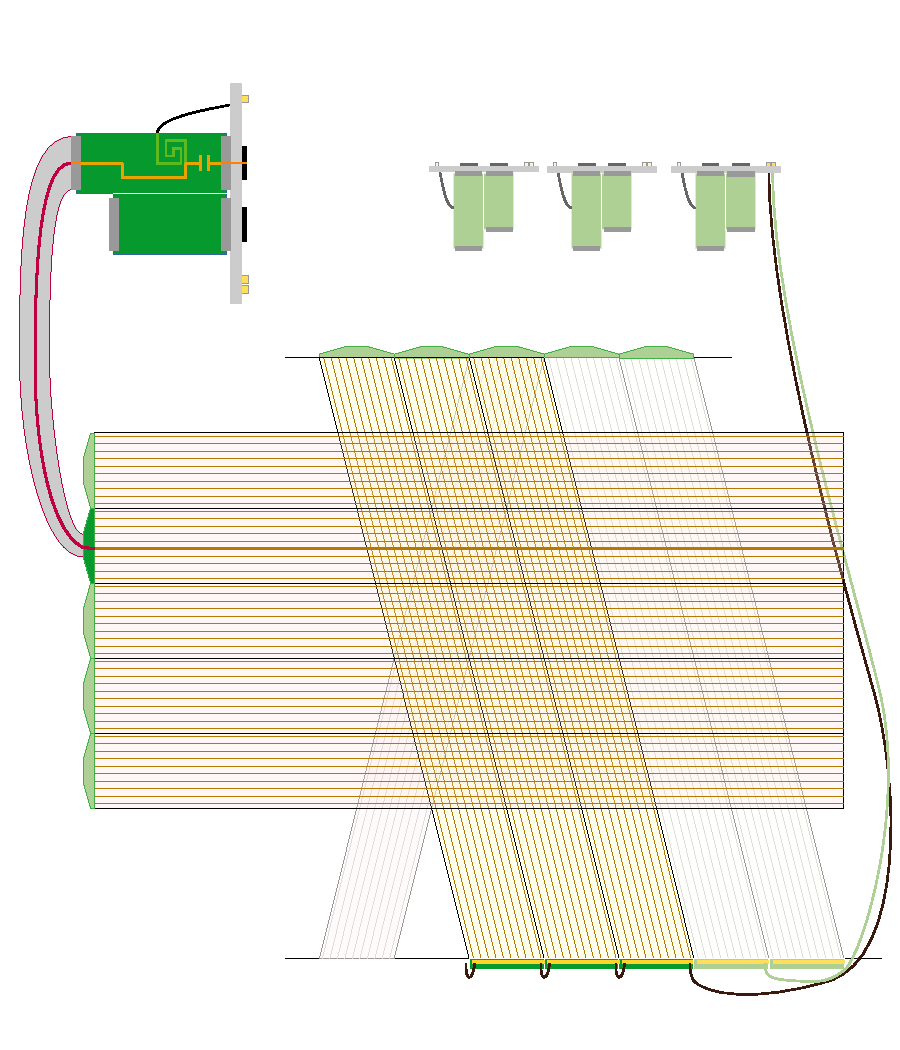
\includegraphics[height=6cm,clip,trim=0 30 0 0]{fig/PulseCableHorizontalPath}\\
  }
  \caption{\label{fig:WireToReadoutInduced}
    Illustration of the path of the test signal for the first induction plane
    wires.
  }
\end{figure}
It should be noted that in this configuration all the 1056 wires of the half
plane are pulsed at the same time. This increases the amount of cross talk
between the 68-wire cables.
\\
No connectivity test was performed on the $\approx 4000$ short wires shown in
\cref{fig:WireCategories} as red category.


\subsection{Test setup}
\label{ssec:methodology:setup}

The test pulse is generated with a ``test box'' designed by Mark Convery
(\cref{fig:TestBox}), which includes a pulse generator and also provides
amplification of the response to the pulse.
After amplification, the responses are digitized by a four-channel oscilloscope
(\href{https://www.tek.com/datasheet/digital-phosphor-oscilloscopes-0}{Tektronix TDS 3054C})
and sent to a program running on a laptop, which can record them as waveforms
(\cref{fig:TestSetup}).
The path followed by the test pulse is illustrated in the following paragraphs.
\\
\begin{figure}
  {
    \centering
    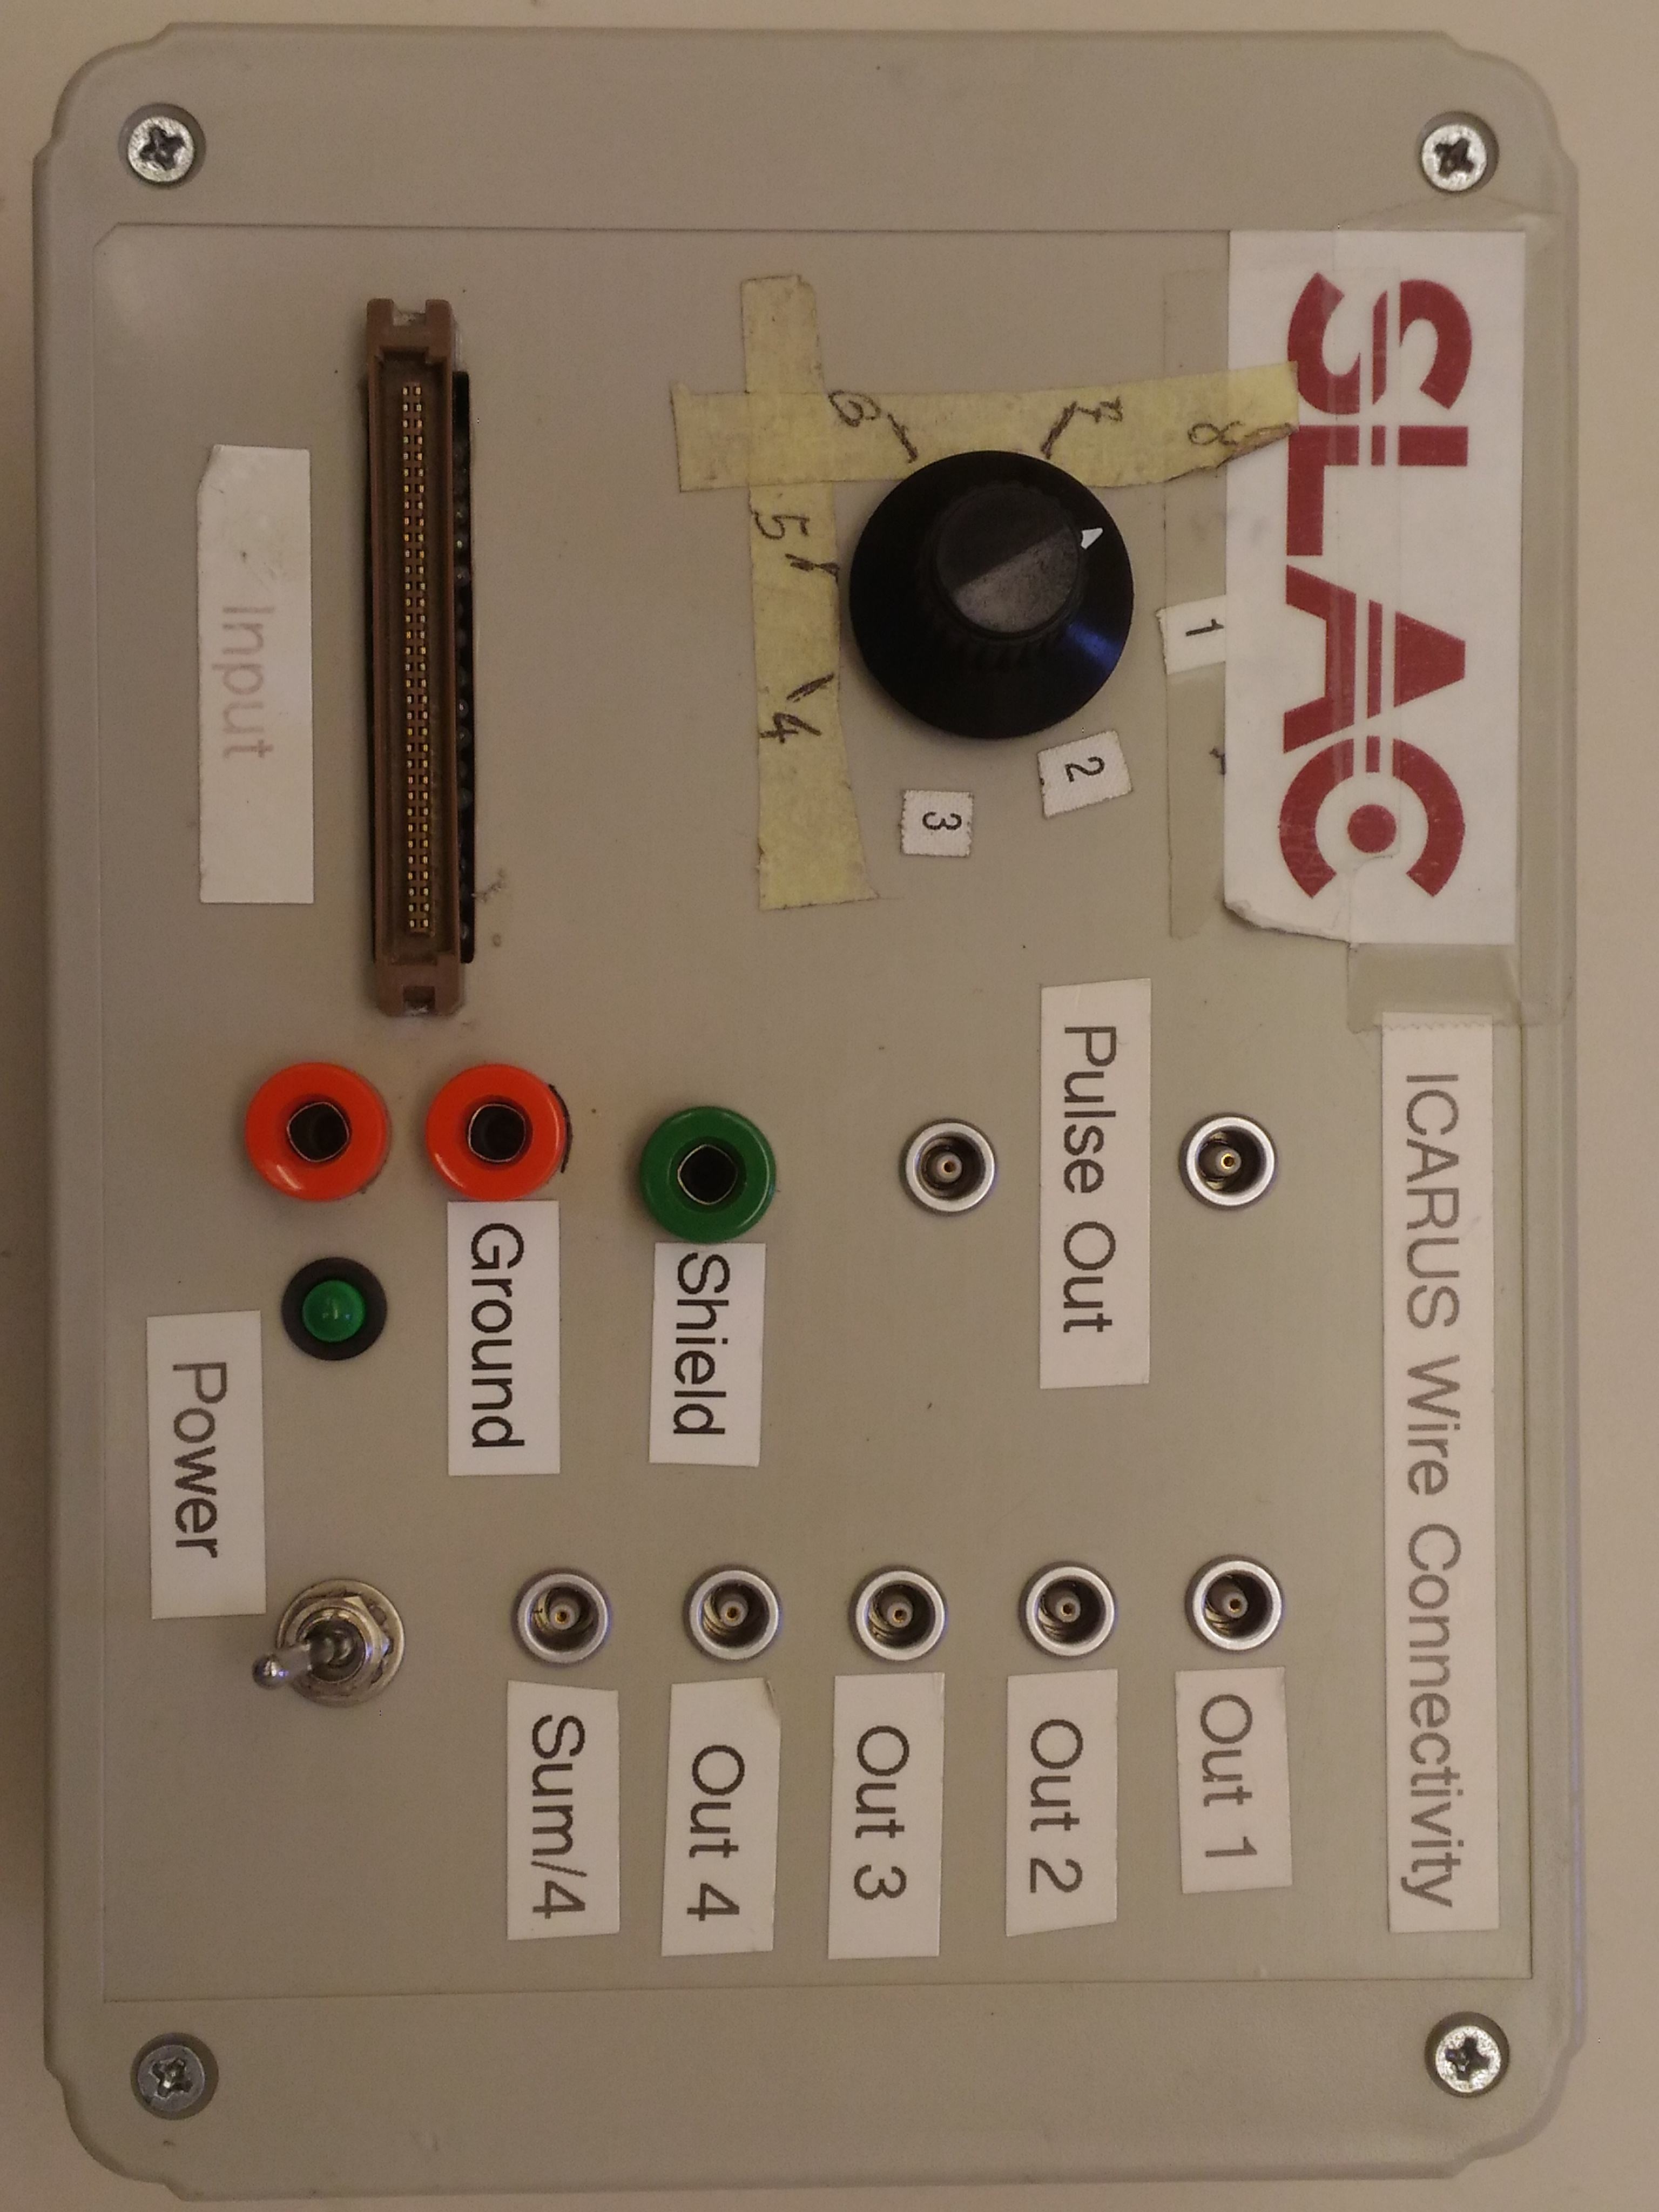
\includegraphics[height=6cm]{fig/20190501_113323-TestBox}\\
  }
  \caption{\label{fig:TestBox}
    The older one of the the two test boxes used for generating the test pulse
    and selecting and amplifying the response to it.
  }
\end{figure}
\begin{figure}
  % there should be somewhere an illustration of the setup...
  \qquad
  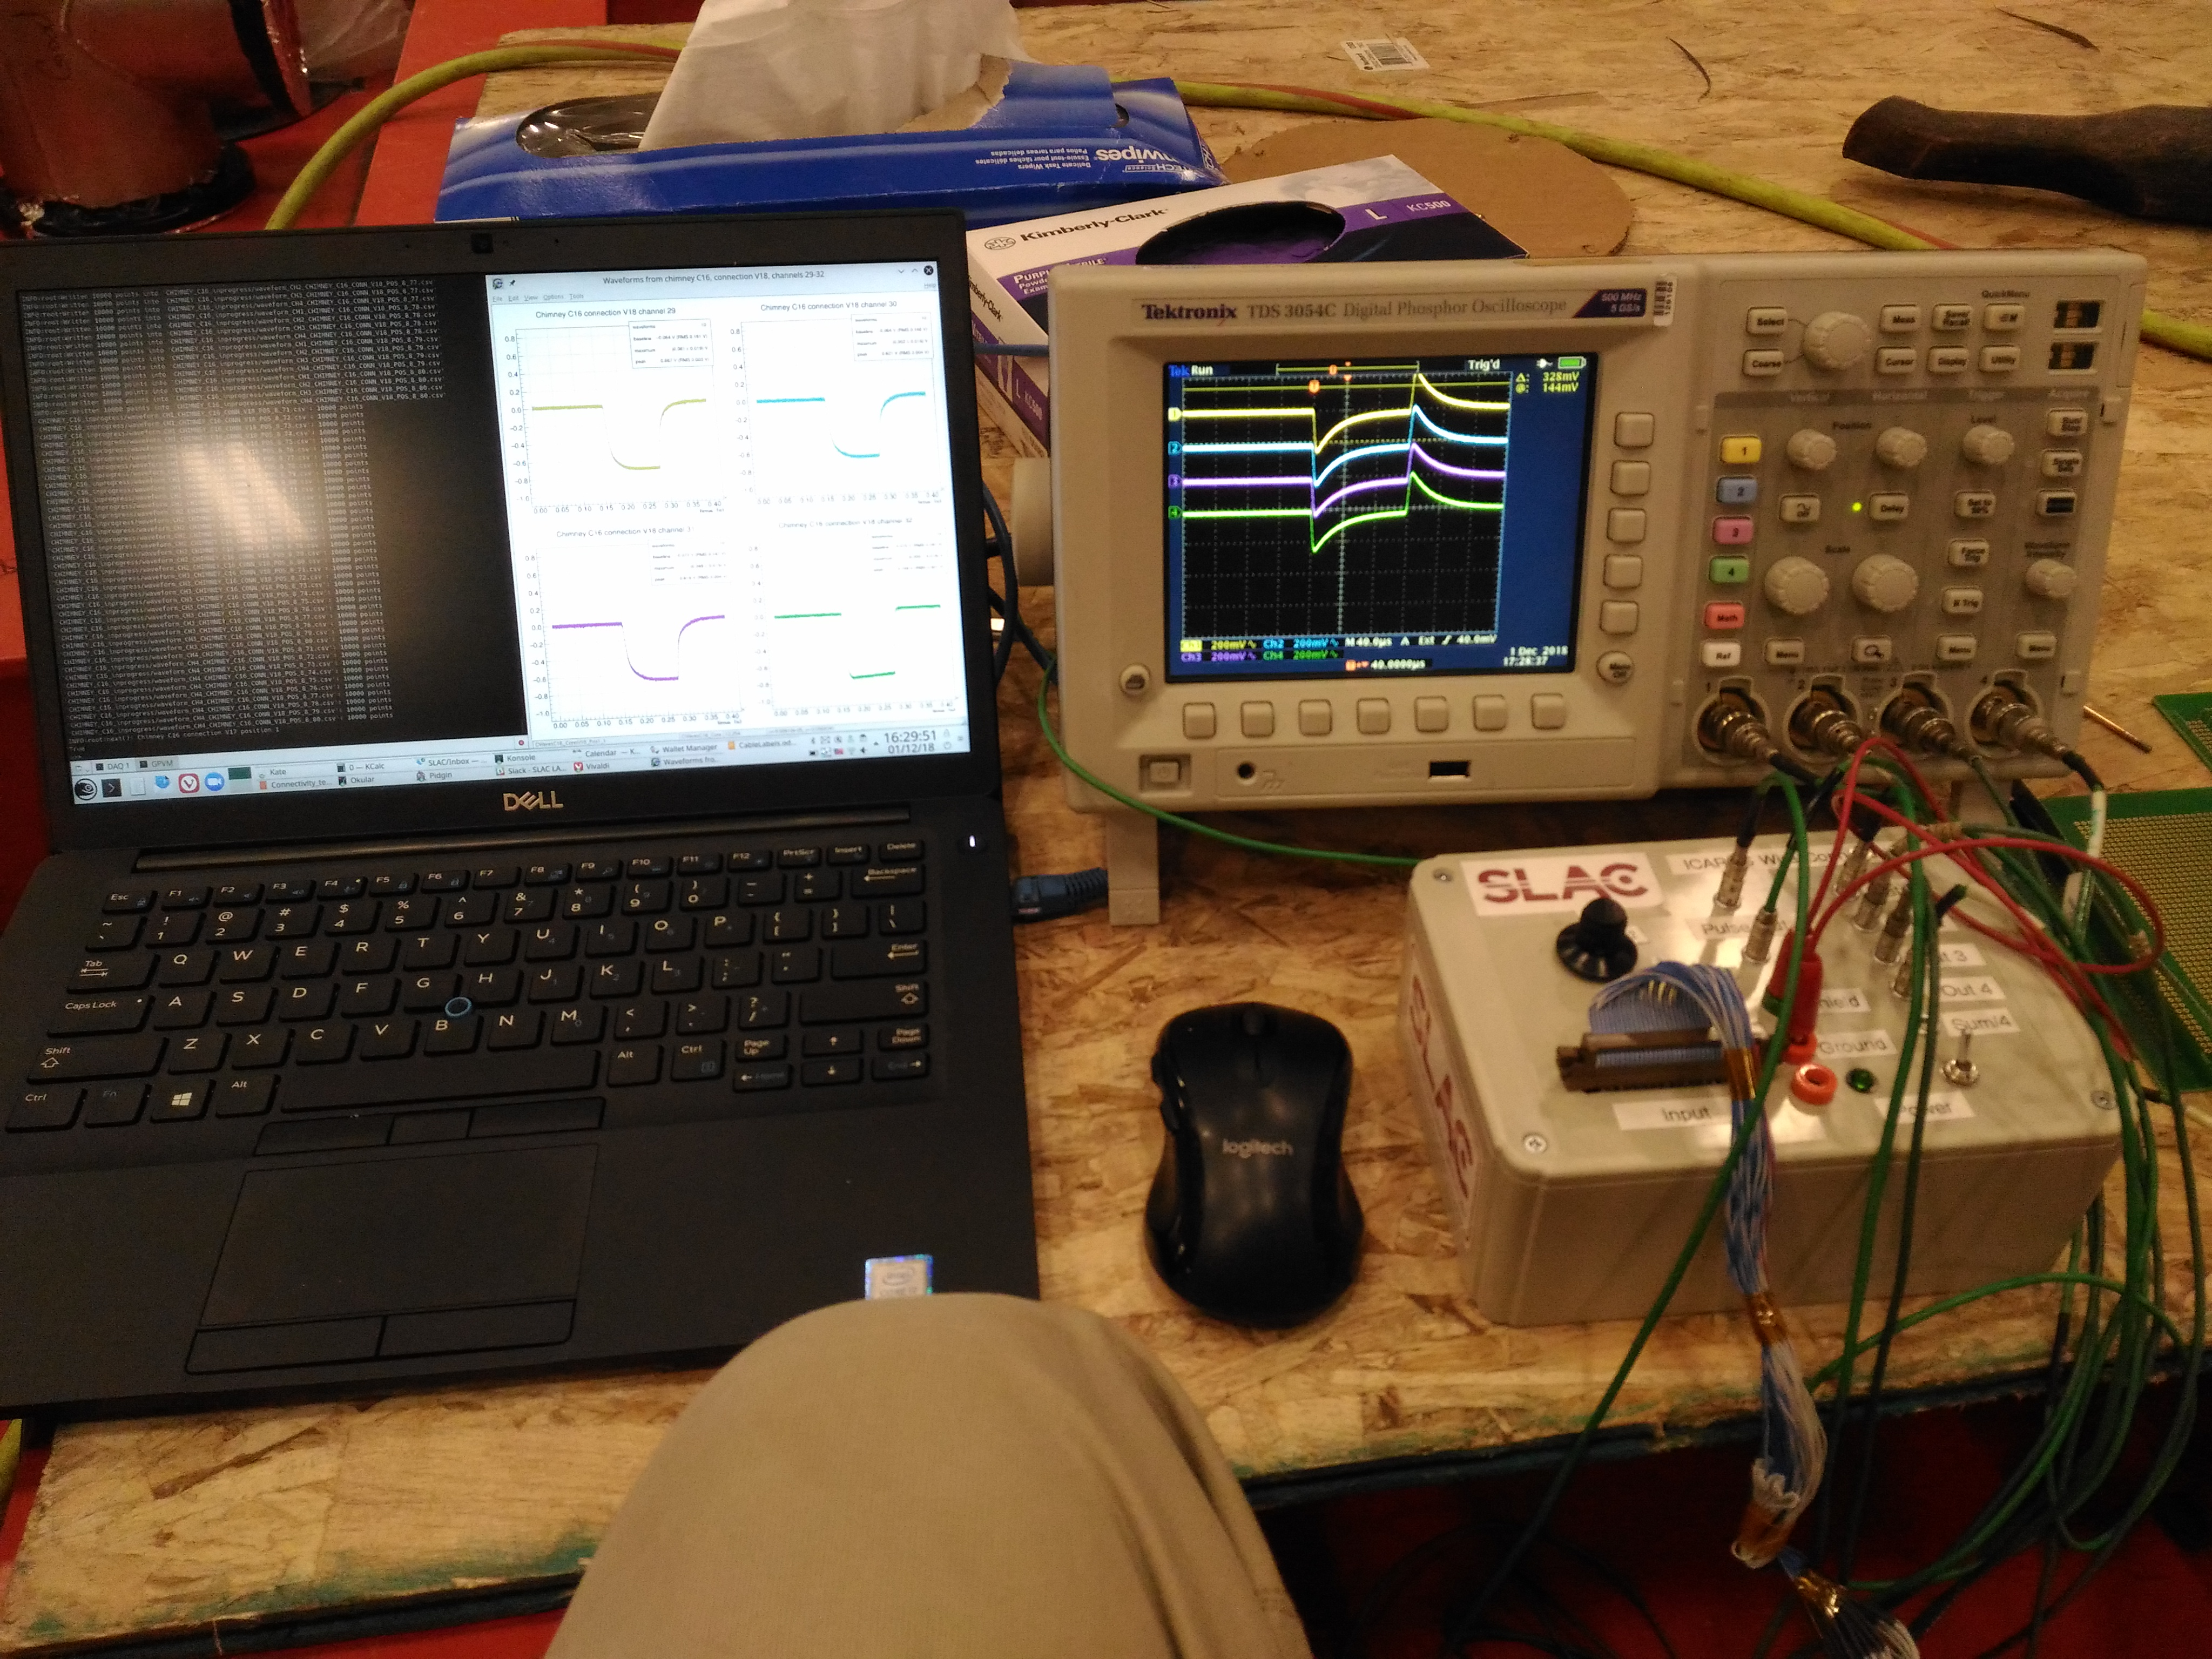
\includegraphics[width=0.48\textwidth]{fig/2018-12-01_16-29-52-ConnectivityTestReadoutSetup}
  \caption{\label{fig:TestSetup}
    Connectivity test readout setup.
  }
\end{figure}
The test boxes are the same used in the testing of September 2018, including the
dead channels (channel 2 in one of the boxes, channel 18 in the other), with
some upgrade.
The boxes are powered by three \V{1.5} AA batteries, and they now include a
voltage regulator that stabilizes the output at about \V{3.3}.
The test pulses are emitted at a rate of \Hz{100}, each one a positive square
wave of \V{3.3} with a duration of about \micros{100}.
\begin{figure}
  \subfloat{
    \raisebox{-0.5\height}{
      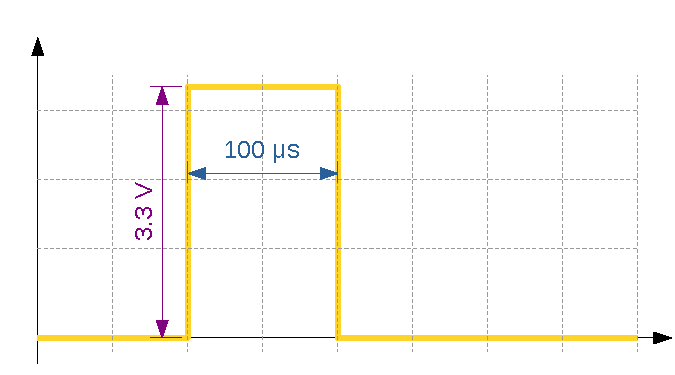
\includegraphics[width=0.48\textwidth]{fig/TestPulseCartoon}
    }
  }
  \subfloat{
    \begin{tabularx}{0.4\linewidth}{ll}
      \hline
      shape          & square wave         \\
      amplitude      & \V{3.3}             \\
      length         & \micros{\approx100} \\
      pulse rate     & \Hz{100}            \\
      \hline
    \end{tabularx}
  }
  \caption{
    Illustration and specifications of the pulse used in connectivity tests.
  }
  \label{fig:TestPulse} 
\end{figure}
Each test box includes two outlets for the same pulse.
One is sent directly to the oscilloscope to work as a trigger.
The other is sent to the detector via a lemo to SMA cable: it will be plugged
either to the test pulse cable or to the bias voltage distribution, to implement
one of the two test paths described in \cref{sec:methodology}.
The response to these pulses is read from the front end connectors on the
flange.
The standard setup includes the installation of an empty readout minicrate, its
only purpose to provide mechanical support, and in it a board shaped as a
readout board, which is in effect just a passive adapter from the front end
connector to a 68 pin cable: each of these ``fake'' readout boards includes two
such adapters, converting at once both the left and the right side connectors,
and allowing for two different 68 pin cables.
At a time, the correct one of the two cables (for example, the left one when the
test is currently pulsing the left bias voltage distribution path) is plugged
back into the test box, conveying signals from the 32 channels from the \DBB
side it is connected to.
The test box contains a eight position switch that selects four contiguous
channels among the 32 from the cable.
Signals from the four channels are amplified and offered each on an independent
outlet.
These four channels are sent to the oscilloscope for digitization and visual
inspection.
The oscilloscope can be driven by commands sent via Ethernet from a laptop,
where a simple data acquisition program drives the readout and recording of the
digitized waveforms.
One of the test boxes also offers ``direct'', non-amplified versions of the
signal.
\\
Noise and grounding have been an issue in the previous session of tests.
Depending on the grounding of the shield wires, they do actually act as shield,
or they rather act as antennas picking up noise.
The upgraded test boxes allow the option of connecting all the shield wires to
the ground (which is effectively the oscilloscope ground).
This option was regularly used in the December 2018 testing session.
It results into reduced noise and also in reduced signal response, allegedly
because of reduction of cross talk from other cables.
In addition, we grounded the oscilloscope chassis to the detector.


\subsection{Data acquisition}
\label{ssec:operations:DAQ}

The Tektronix TDS 3054C oscilloscope can digitize and send out the input
signals, providing $10^4$ samples per channel,
each sample with 8-bit precision\footnote{
The oscilloscope alternatively allows for 9 bit ADC conversion, at the cost of
doubling the data size}.
The custom data acquisition code reads a sequence of waveforms from each
oscilloscope channel.
Each waveform is stored in its own comma-separated value file (CSV),
with a resolution of \micros{0.1} for the time and \milliV{10} for the signal
amplitude. Therefore the waveform samples span 1 millisecond, and they are at
baseline in roughly $60-80\%$ of the time.
\\
The testing procedure included cycling across all 8 switch positions of the test
box for each connection, and recording 10 waveforms for each of the 4 channels
monitored in the selected position. For each switch position, therefore,
40 waveforms are recorded. The total data size as stored in the final form is
about \mebiB{500} per chimney.


\subsection{Labelling}
\label{ssec:labelling}

\begin{figure}
  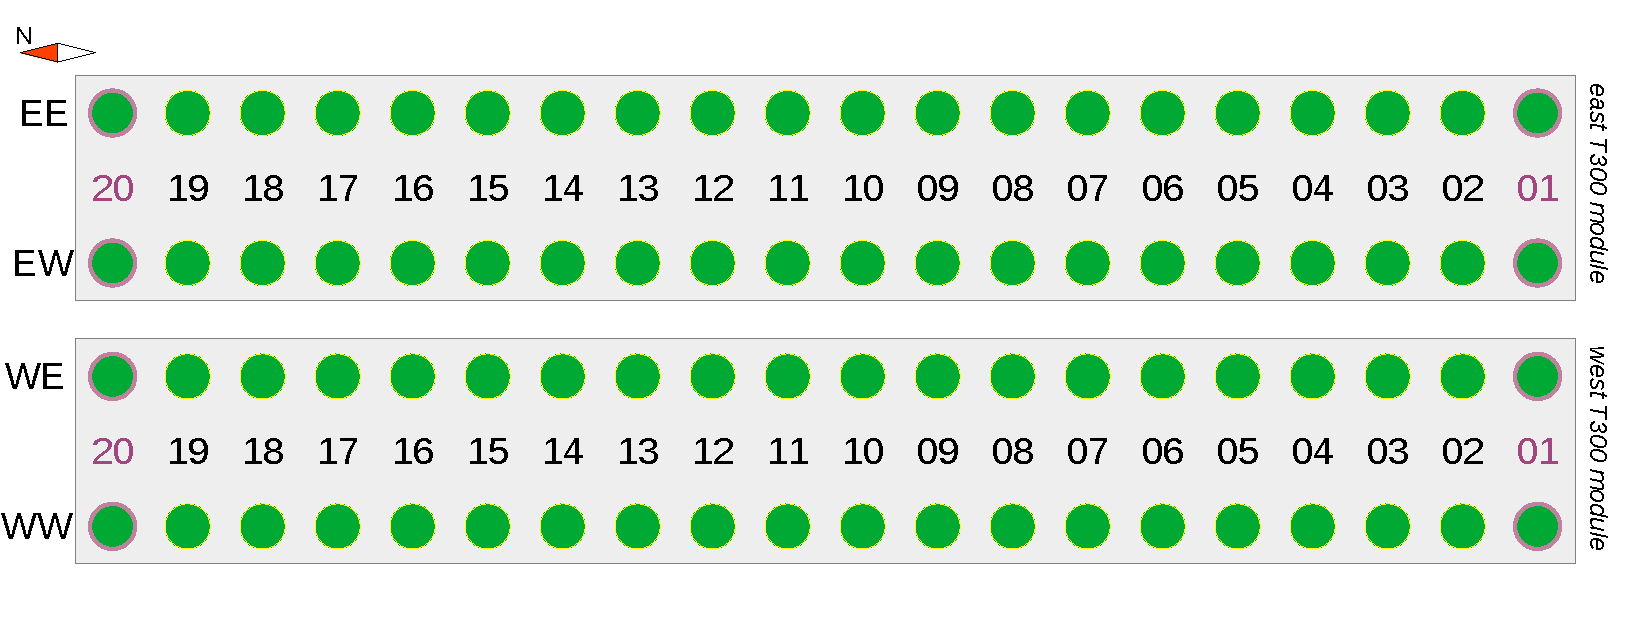
\includegraphics[width=\textwidth,clip,trim=0 35 0 10]{fig/ChimneyMap}
  \caption{\label{fig:ChimneyLabelling}
    Disposition and labeling of the chimneys. End chimneys (\texttt{01} and
    \texttt{20}) are circled in magenta.
  }
\end{figure}

We use the following labeling conventions:
\begin{description}
  \item[chimneys] are laid out in four ``columns'' and twenty ``rows'':
    \begin{itemize}
      \item columns are labeled geographically, with the position of the module
            first (\texttt{E}ast or \texttt{W}est) and then the side within the
            module (also \texttt{E}ast or \texttt{W}est)
      \item rows are numbered \texttt{01} (the most northern one) to \texttt{20}
            (the most southern one, the side neutrino beams come from)
    \end{itemize}
    Chimneys \texttt{01} and \texttt{20} are taller and host three flanges,
    and they have been called ``end'', ``corner'', or ``tall'' chimneys;
  \item[flanges] are rarely referred to directly; we'll use the letter
    \texttt{F} followed by the flange number, that effectively went from 1 to
    100 (there are 96 flanges mounted on the detector, but spares were produced
    as well)
  \item[cables] (68-wire cables) are numbered from \texttt{01} to \texttt{18},
    except for the ones serving the first induction plane, where the range
    extends to \texttt{33}; the cables have a letter tag too, which can be
    \texttt{V} (east side of each module), \texttt{S} (west side of each
    module), or \texttt{A}/\texttt{B}/... in the end chimneys; since this cable
    tag does not add any information, occasional inconsistencies are
    nonconsequential
  \item[channels] and wires are usually identified by a number between 1 and 32
    within each cable, with channel 1 being the one marked by the red wire on
    the cable itself. In connectivity test context, a 4-channel oscilloscope
    is used for digitization, and a channel $c$ might be designed by test box
    switch position ($p$) and oscilloscope channel ($CH$) instead: the numerical
    rule is $ c = 1 + 4 (p - 1) + (CH - 1) $
  \item[position] of the switch in the test box spans the range 1--8, where
    position 1 covers channels 1 to 4, position 2 covers channels 5 to 8, up to
    position 8 covering channels 29 to 32
  \item[oscilloscope channel] is one of the four channels of the oscilloscope;
    we use to color-code them as yellow (CH1), cyan (CH2), green (CH3) and
    magenta (CH4), after the color the oscilloscope associates them to. In
    general it is recommended that the channel as defined above is used instead,
    which is not bound to this specific test.
\end{description}




% \section{Waveform analysis}
\label{sec:Analysis}


A fast data analysis was performed within hours or days from the data
acquisition. Each waveform is analysed individually, through a few
steps:

\begin{itemize}
\tightlist
\item
  baseline identification: average of the central 50\% of the samples
\item
  RMS: RMS of the samples used in the baseline determination
\item
  extrema determination: amplitude of the positive and negative peaks
  along the whole waveform
\end{itemize}


For each channel, the parameters from all the available waveforms (10)
are averaged to extract:

\begin{itemize}
\tightlist
\item
  baseline RMS (RMS of the 10 baselines)
\item
  noise average (average of the 10 RMS, one for of each baseline)
\item
  peak amplitude average and its uncertainty (the positive
  peak from each waveform are averaged)
\end{itemize}

This analysis is aimed for speed, and it can definitely be refined.

% ----------------------------------------------------------------------
\subsection{Baseline and RMS identification}
\label{sec:baseline-and-rms-identification}


The principle is to exclude the signal, intended as the response to the
pulse, and to use the remaining of the waveform to estimate the
baseline. The algorithm is designed not to require prior knowledge of
the position or shape of the peaks.\\

The signal is shaped as two sharp-rising peaks, which including the
decay tails are roughly 200 µs or shorter. The algorithm relies on the
assumption that those two peaks are indeed roughly that narrow, although
it does not assume anything on their size or shape. It flows as follows:

\begin{enumerate}
\tightlist
\item
  sort all the 10000 samples in increasing order; in this way, the
  samples taken during the negative peak will be at the left of the
  data, the ones at the positive peak will be at its right, and the
  middle of the data will be populated by long sequences of samples with
  similar values, from the baseline
\item
  select the samples from \#2500 to \#7499 from the sorted data for
  further analysis
\item
  take the average and RMS of the selected samples, which will represent
  the baseline and noise respectively
\end{enumerate}

This algorithm may present some bias if the tail from the first peak
overlaps the second peak. An alternative, simple algorithm would rely on
the assumption that the peak is on the second half of the waveform, and
would therefore use the first 40\% or 50\% of the waveform for baseline
determination as in the last point of the algorithm.\\

An older version of the algorithm would rely of the knowledge of the
peak position, and would fail when the waveform does not contain any
actual signal.


% ----------------------------------------------------------------------
\subsection{Peak determination}
\label{sec:peak-determination}


Again a simple algorithm, the peak determination consists of two simple
steps:

\begin{enumerate}
\tightlist
\item
  determine the absolute maximum and minimum of the waveform
\item
  subtract to both the baseline (obtained separately)
\end{enumerate}

This algorithm is affected by the noise on the waveform, which can be
quantified together with the baseline. Although this is less than ideal,
the actual noise has been measured to be low enough to be not
significant for the purpose of the fast analysis we performed{[}1{]}.\\

{[}1{]} In more recent versions of the library, the minimum and maximum
are not evaluated from the single sample, but replaced by a running
window average on 5 samples.


% ----------------------------------------------------------------------
\subsection{Results}
\label{sec:results}

We summarize the results of the baseline, RMS, positive peak value, 
and the ratio of the positive peak value to the baseline in 
\Cref{fig:baseline,fig:rms,fig:pospeak,fig:pospeaktobaseline}.
Each strip represents a single channel of the detector.
The x-axis includes all the chimneys of the ICARUS detector, while
the y-axis shows all the 18 cables, each with 32 channels, within a chimney.
The color code in each figure indicates the values of the baseline, the RMS,
the positive peak, or the ratio of the positive peak value to
the baseline value.\\

The corner chimneys, Ch01 and Ch20 in each row, have only the channels
connecting to horizontal wires, where the data was not recorded in this
round of the connectivity test and therefore is not shown in the plots.
Cables 1-9 in Ch02 and Ch03 and cables 10-18 in Ch18 and Ch19 are connected
to the corner wires in the second induction and collection planes which are
shorter in length.
Owing to their ending points, the cables injecting the test pulse are
not located at the same chimney.
Without the information of the location of the pulse-injecting cables,
we are not able to obtain a result of these wires, and 
\Cref{fig:pospeak,fig:pospeaktobaseline} show extremely low or
overflown values.\\


% ----------------------------------------------------------------------
\begin{figure}
\centering
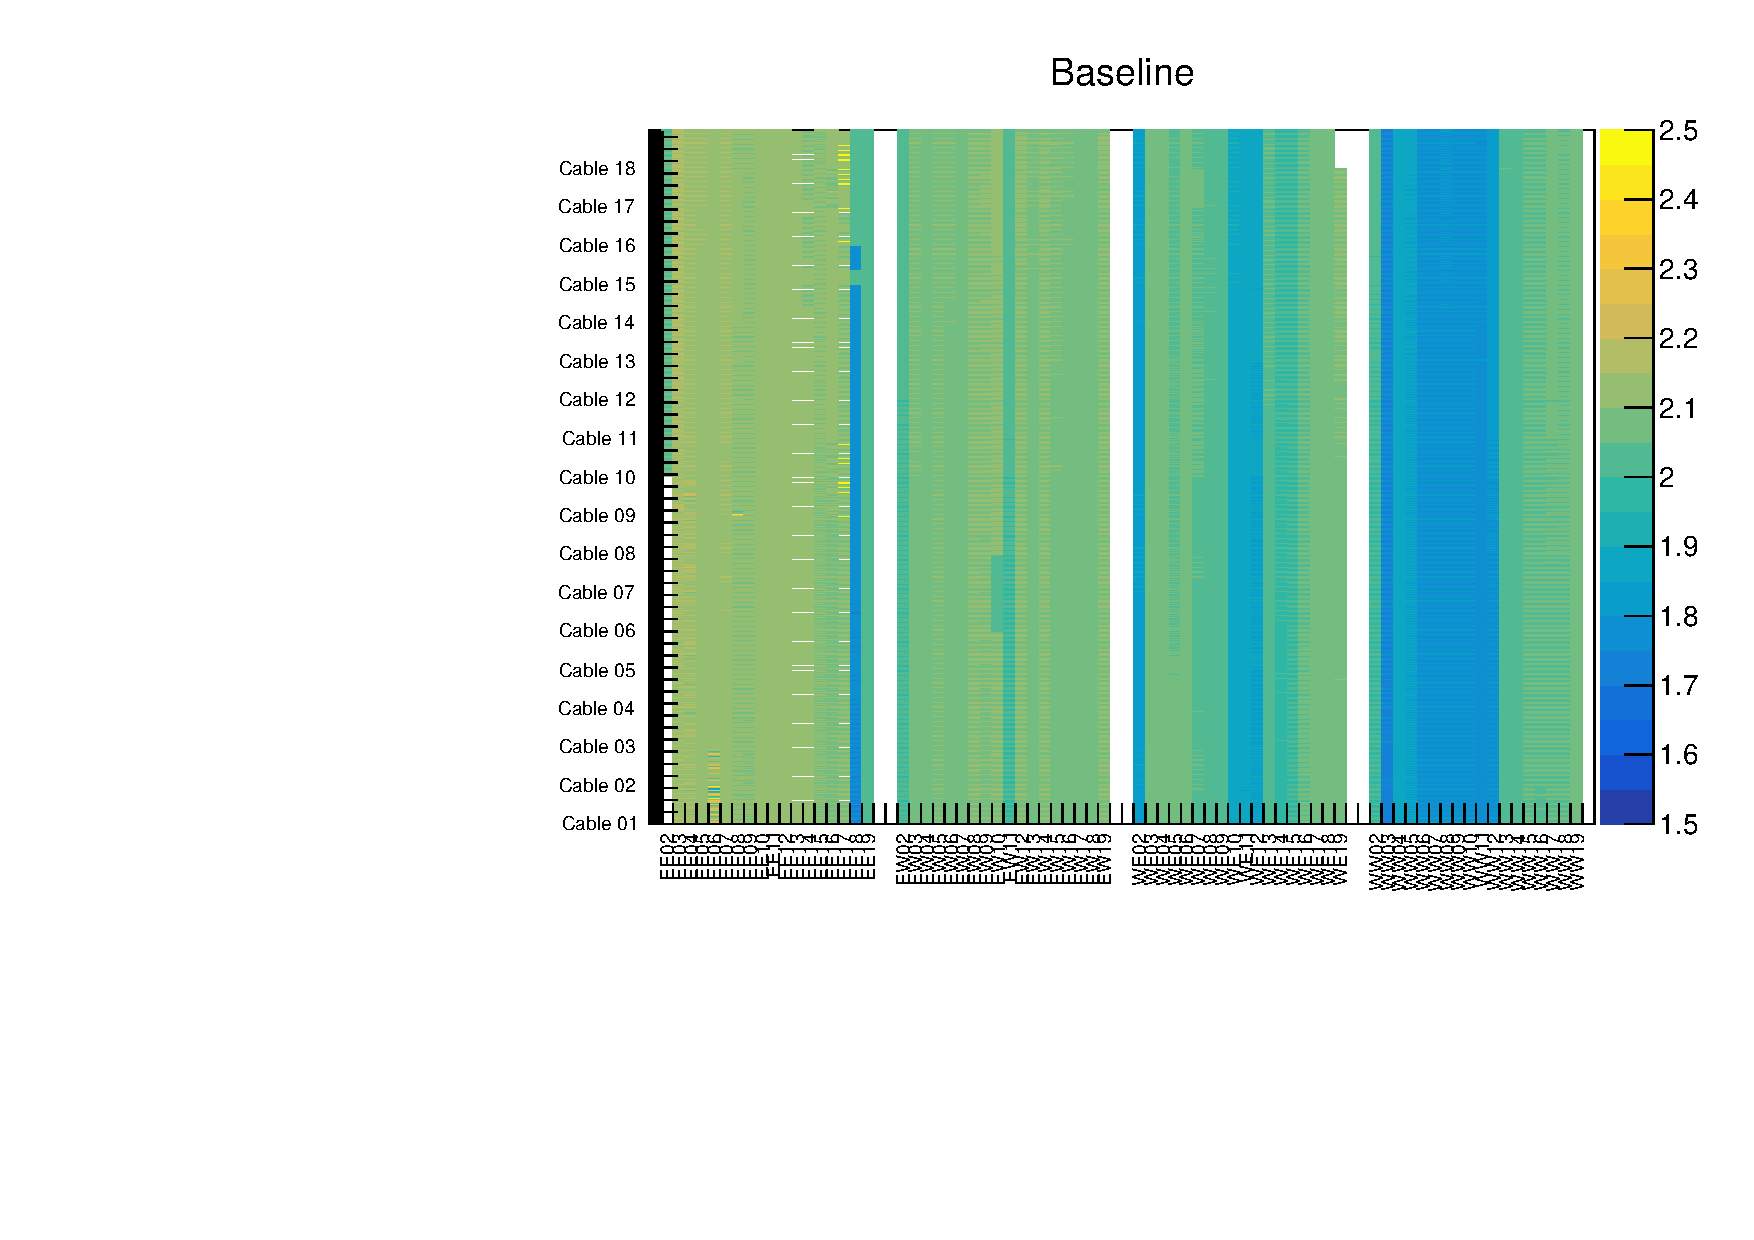
\includegraphics[width=\textwidth]{fig/Baseline.pdf}
\caption{The map of the baseline values of all the channels.
Each strip represents a single channel of the detector.
The x-axis includes all the chimneys of the ICARUS detector, while
the y-axis shows all the 18 cables, each with 32 channels, within a chimney.
The color code in each figure indicates the values of the baseline.}
\label{fig:baseline}
\end{figure}
% ----------------------------------------------------------------------

% ----------------------------------------------------------------------
\begin{figure}
\centering
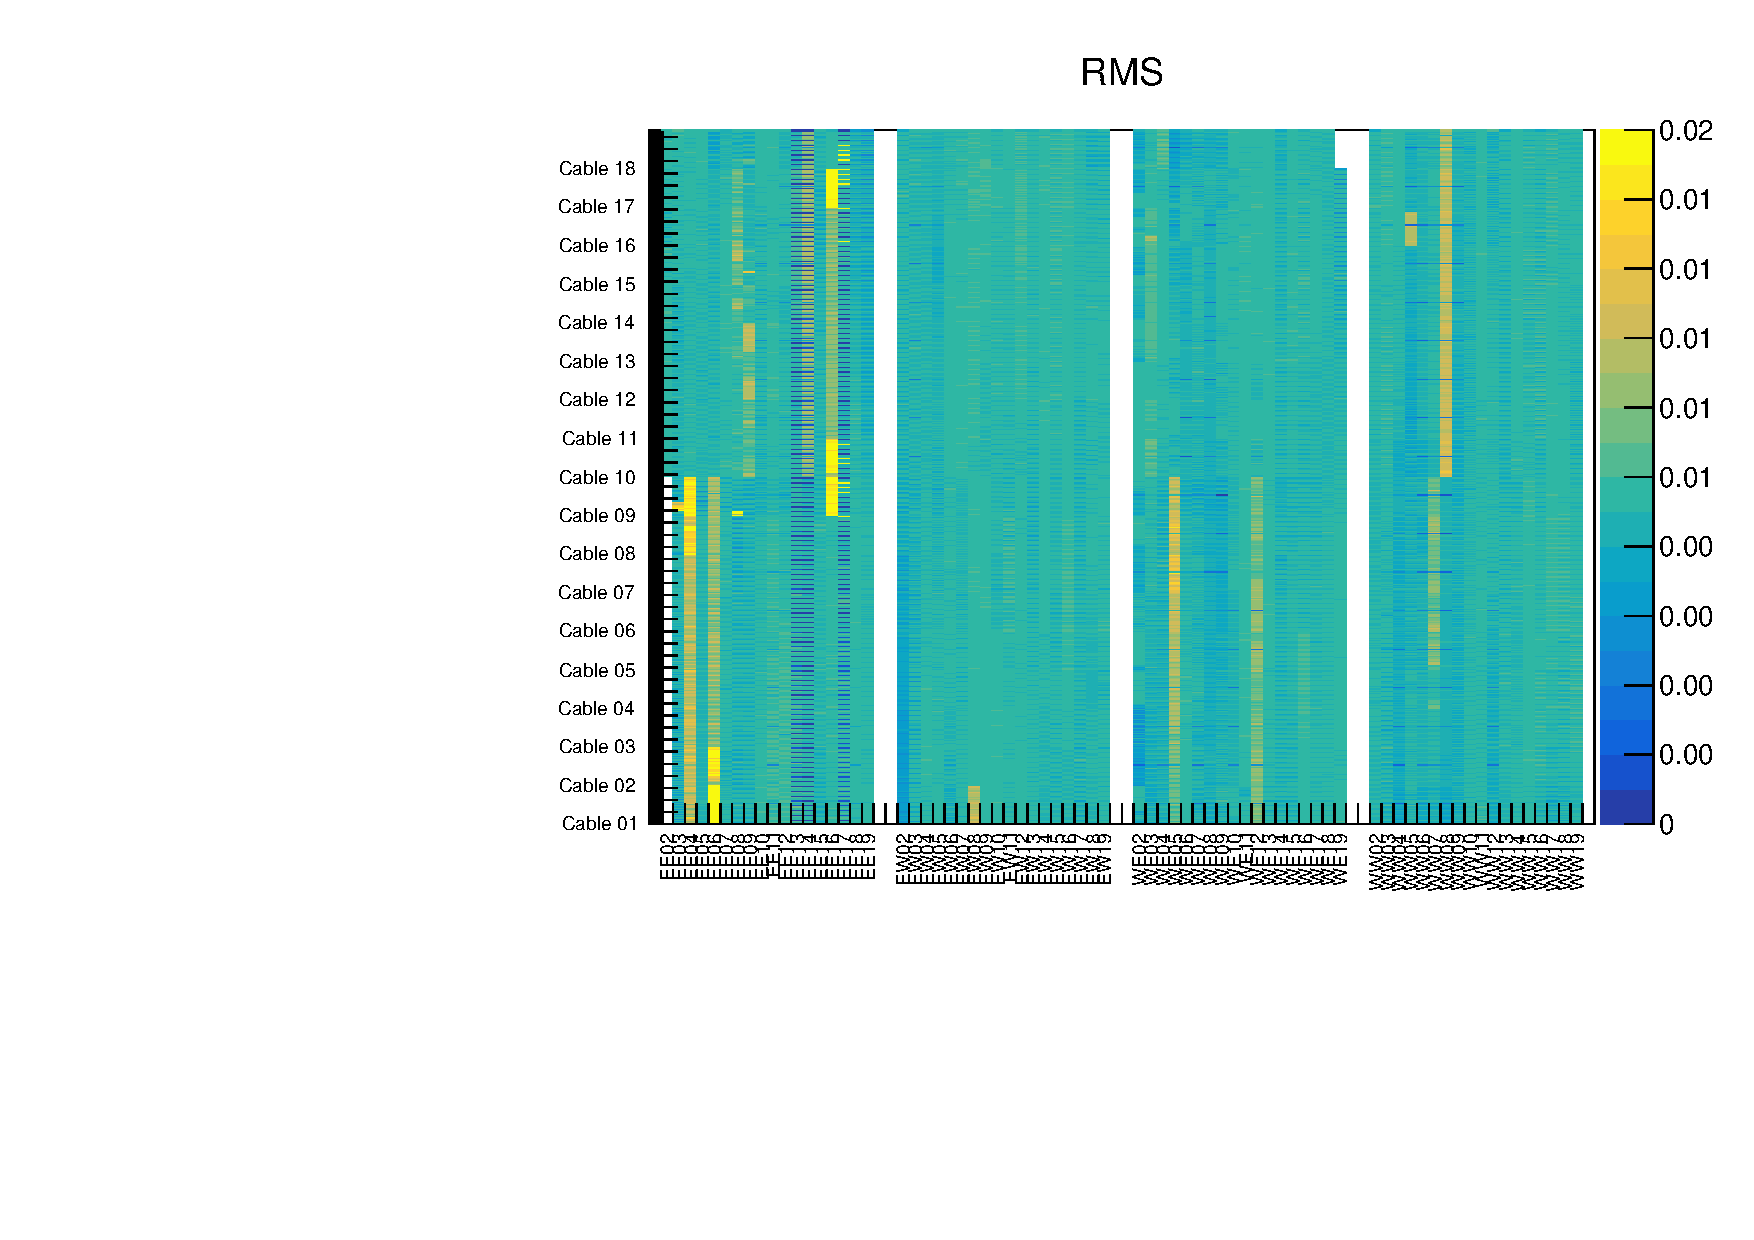
\includegraphics[width=\textwidth]{fig/RMS.pdf}
\caption{The map of the RMS of all the channels.
Each strip represents a single channel of the detector.
The x-axis includes all the chimneys of the ICARUS detector, while
the y-axis shows all the 18 cables, each with 32 channels, within a chimney.
The color code in each figure indicates the values of the RMS.}
\label{fig:rms}
\end{figure}
% ----------------------------------------------------------------------

% scale in the oscilloscope
In chimneys EE13, EE14, and EE17, the white strips in \Cref{fig:baseline} 
and the dark blue strips in \Cref{fig:rms,fig:pospeak},
indicating extremely low values,
appear in every four channels.
It is owing to the fact that the fourth channel in the oscilloscope
happens to be set a larger scale in voltage, and, as a consequence, 
the relative values of the baseline and the pulse peak are small.
The effect is canceled out in \Cref{fig:pospeaktobaseline}, where the
ratio of the peak to baseline values is plotted.\\

% dead channel in the test box
The fifth channel of the connector for the flat ribbon cables in a test
box is damaged, and we are not able to read out the signals from the
channel when using this test box.
It thereby shows the dark blue strips in chimneys EE10-14, EW 03-07,
WE02-12, and WW03-12 in \Cref{fig:pospeak,fig:pospeaktobaseline}.
Nonetheless, this round of the connectivity test aims to identify
potential problems in terms of cables, and a single damaged channel
in the test box should not affect the effectivity.\\

% voltage
Since there is no voltage regulator for the battery powering the test
boxes, the baseline value, which is set to the half of the voltage,
decreases as the time being, as shown in \Cref{fig:baseline}.
Hence, \Cref{fig:pospeaktobaseline}, which cancels out the baseline
decrease, gives us a more uniform comparison across the whole detector.\\

% special cables
In the EE and WE rows, cables 1-8, cable 9, cables 10-17, and cable 18
have separate pulse-injecting cables, while in the EW and WW rows, those
groups are cable 1, cables 2-10, cable 11, and cables 12-18.
During the tests, we do not have the information on this grouping of
wires, except that cables 1-9 and 10-18 are for induction and collection
wires, respectively, and have different pulse-injecting cables.
Consequently, for some chimneys, cables 1-9 are tested with
the same pulse-injecting cable, and so are cables 10-18; 
for other chimneys, cables 1-8, 10, 11-17, and 18 are tested with different
pulse-injecting cables.
With the cross talk effect discussed in the next paragraph,
it is not straightforward to distinguish whether the measured signal
corresponds to the injected pulse or the cross talk signal in the special
cables, cables 9 and 18 in the EE and WE chimneys and cables 1 and 11
in the EW and WW chimneys.
In addition, it is raised that the grouping of the channels for the same
pulse-injection cables might be cables 1-8, 9, 10-17, 18 for the chimney
EE02, but cables 1, 2-10, 10-17, 18 for the next chimney, EE03, and
similar patterns for other chimneys.
However, we have not reached a conclusive statement by analyzing the
current data, which convolved several issues including the cross talk,
potentially wrong cables for pulse-injection, etc.
We defer the conclusion to the next iteration of connectivity test
where we expect to have equipment disentangling those issues.\\

% cross talk
The wires involved in the connectivity test should normally not be connected
to the detector ground, but it was observed that some of them are during the
overhaul at CERN.
The design of the test box in this iteration does not connect the wire cables
to the detector ground, and therefore in the normal case of the wire grounding,
the cross talk from the adjacent twisted wires contributes a significant
portion to the signal.
Roughly speaking, the amplitude of the cross talk signal is similar to
to that of the injected pulse, which severely complicates the signal
interpretation.
In the normal case, where the wire is correctly connected but not grounded 
to the detector, the signal will be the superposition of the injected
pulse and the cross talk signal.
On the other hand, in the cases that the wire is not connected and not
grounded, and that the wire is connected and also grounded,
the signal will contain, respectively, only the cross talk and only the
injected pulse, both of which will have roughly half the amplitude of
the signal in the normal condition.
By analyzing all the possible scenarios listed in \Cref{table:crosstalk},
we ensure the connectivity of the channels with the full size amplitude in
\Cref{fig:pospeaktobaseline}.
Further, to distinguish the connected wires among those with the half 
size amplitude, such as cable 8 in chimney WW06, cables 4 and 17 in chimney WW12,
we explicitly check their grounding.
The check confirms those wires are grounded and we are reading the injected
pulse but not the cross talk from adjacent wires.\\

\begin{table}
\centering
\begin{tabular}{ccc}
\hline
\hline
    & Shield grounded  & Shield isolated \\
\hline
Cable connected & 1/2 size signal & Full size signal \\
Cable disconnected & No signal & 1/2 size signal \\
\hline
\hline
\end{tabular}
\caption{The qualitative signal amplitudes of all the
possible scenarios of shield grounding and
wire connection.}
\label{table:crosstalk}
\end{table}


% ----------------------------------------------------------------------
\begin{figure}
\centering
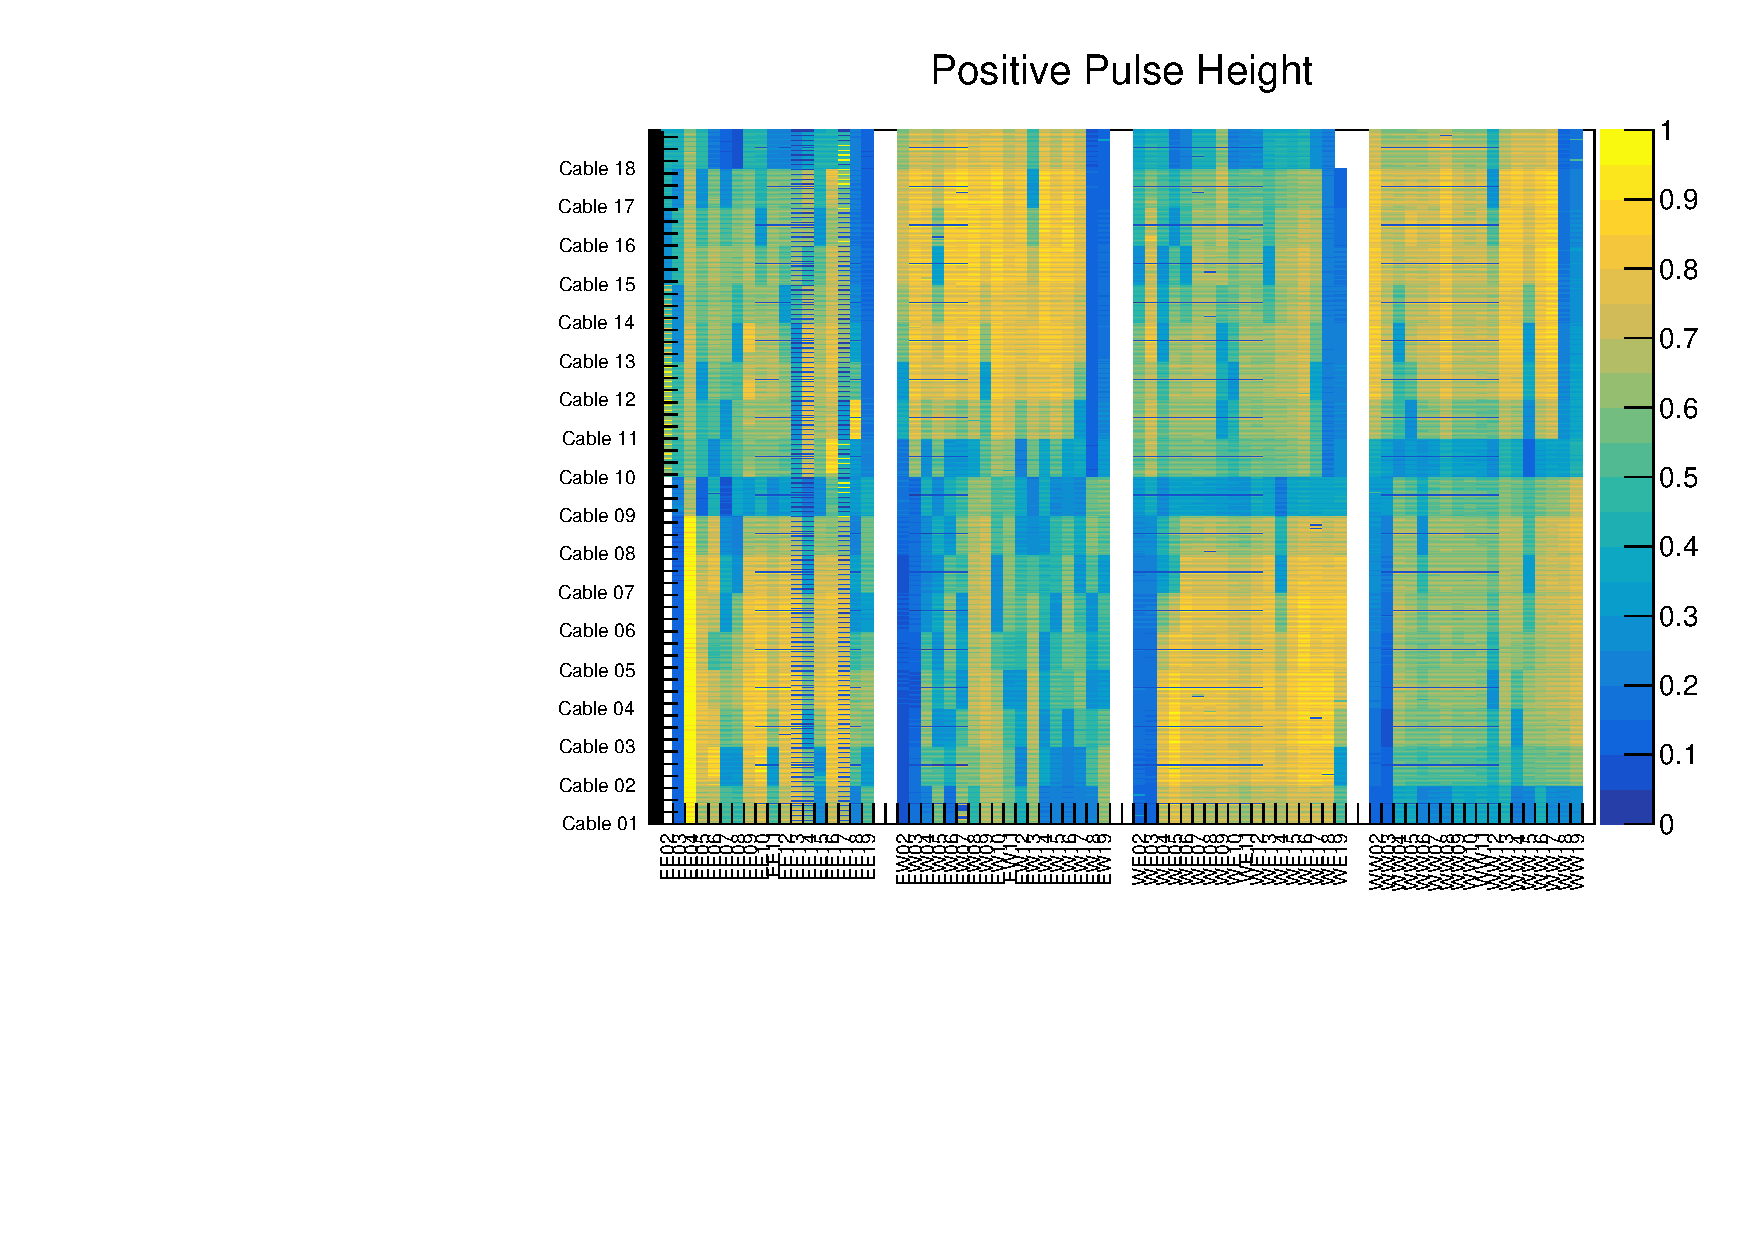
\includegraphics[width=\textwidth]{fig/PosPeak.pdf}
\caption{The map of the positive peak values of all the channels.
Each strip represents a single channel of the detector.
The x-axis includes all the chimneys of the ICARUS detector, while
the y-axis shows all the 18 cables, each with 32 channels, within a chimney.
The color code in each figure indicates the values of the positive peak.}
\label{fig:pospeak}
\end{figure}
% ----------------------------------------------------------------------

% ----------------------------------------------------------------------
\begin{figure}
\centering
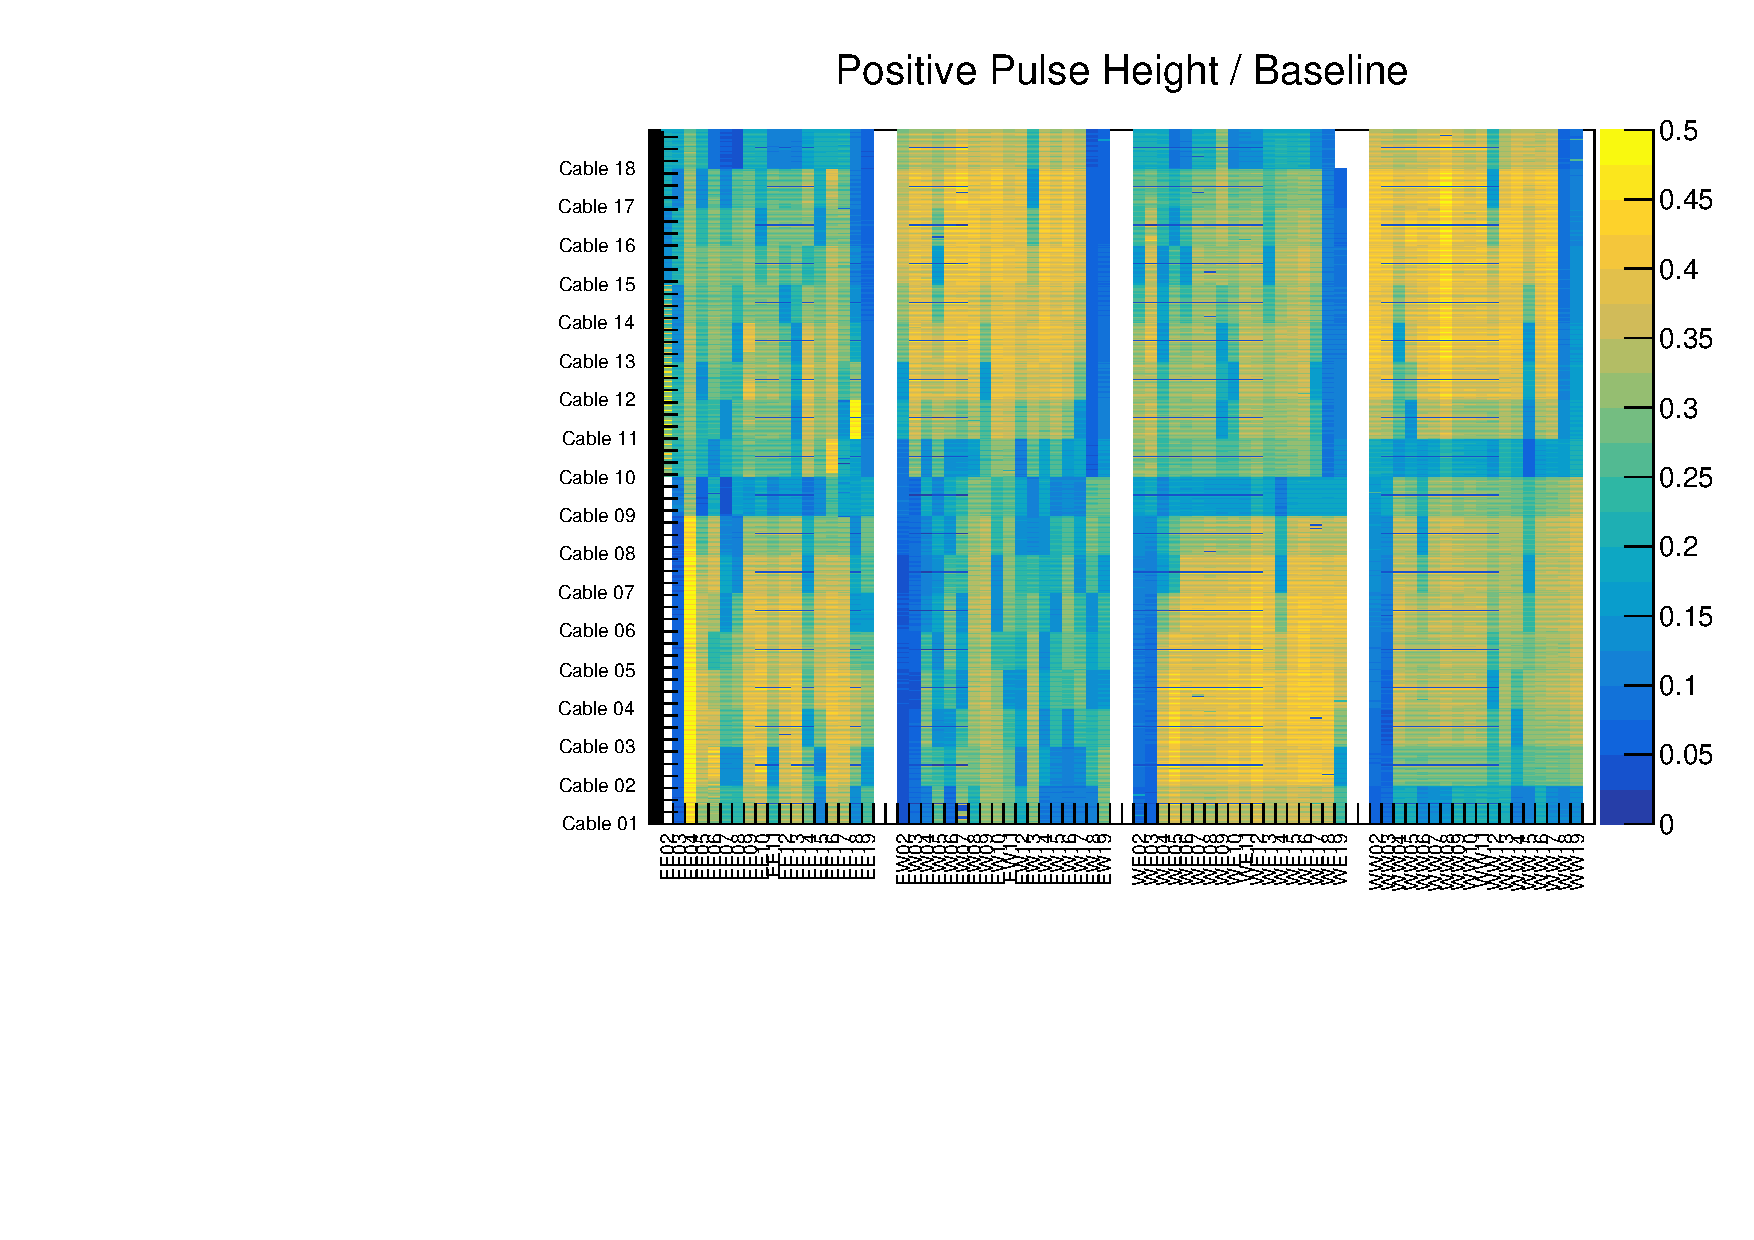
\includegraphics[width=\textwidth]{fig/PosPeakToBaseline.pdf}
\caption{The map of the positive peak to baseline ratios of all the channels.
Each strip represents a single channel of the detector.
The x-axis includes all the chimneys of the ICARUS detector, while
the y-axis shows all the 18 cables, each with 32 channels, within a chimney.
The color code in each figure indicates the values of the ratio.}
\label{fig:pospeaktobaseline}
\end{figure}
% ----------------------------------------------------------------------

% fine structure in the same cable
\Cref{fig:pospeaktobaseline} shows slight non-uniformity
in the signal amplitude of some cables, 
such as cables 10-13 in chimney EE09.
Looking into the values of those cables, we clarify those cables do not
have particularly non-uniform signal amplitudes, and the effect shown
in \Cref{fig:pospeaktobaseline} is rather owing to the color scale.\\

% conclusion
We conclude that there is no disconnected cable, and the source of all 
the cables with lower signal amplitude is confirmed to be the grounding.




\section{Interpretation of the results}
\label{sec:Results}

Histograms, shielded/non-shielded cable problems, cross-talk, etc....



\appendix

\section{Operative details}
\label{sec:operations}


The tests subject of this report happened in three distinct sessions:
\begin{description}
  \item[December 2018] the first extensive test including the \DBB and flanges
    took place. All mounted chimneys were eventually covered in three weeks,
    and the data from the test was recorded.
    This excludes \Chimney{WE02}, \Chimney{WE03}, \Chimney{WE04} and
    \Chimney{WW02}, which at that time were not physically available yet.
  \item[February 2019] another session was scheduled and took place in February
    2019, with the goal of performing the test in the final chimney
    configuration; it was split in two subsessions because for half of the
    chimneys optical flanges were going to be installed, and that installation
    could accidentally impact the connections of the other components in the
    chimney. All the chimneys were again tested, but the only recorded data
    was for the few chimneys that were missing it from December 2018.
  \item[March 2019] saw the last session take place, after an extensive
    intervention on all flanges to deposit glue on the clamps holding the
    68-wire cables.
\end{description}


The following sections describe contributions to the test shifts of the
different sessions.
In addition to those, invaluable contributions on many different levels
have been provided by a very large number of people.
Among others, Alberto Braggiotti, Sandro Centro, Angela Fava, Alberto Guglielmi,
Connie Meng, Claudio Montanari, Donatella Torretta, Zachary Williams
and others that we are surely forgetting to list here but who were nonetheless
crucial to the success of the test.


\subsection{December 2018 test}
\label{ssec:operations:December2018}

The session took place between December 1 and 21, 2018.
The goal of the test was to test all channels served by the 72 short chimneys,
plus all the channels from the first induction wire plane. The session fell
short of that goal because of some of the chimneys were not installed by the end
of the test time window.

Both the test through the test capacitance and through the bias voltage feed
were systematically performed, but only the data from the test capacitance test
was recorded, covering the channels from all the tested chimneys.

Resources (documentation material, communication, ...) include:
\begin{itemize}
  \item SBNFD electronic logbook (\href{http://dbweb6.fnal.gov:8080/ECL/sbnfd/E/search?id=&id_from=&id_to=&t_after=12\%2F01\%2F2018&t_before=12\%2F24\%2F2018&tag\%3AReadout+Testing=on&action=Search}{tag: \emph{Readout Testing}});
  \item \href{https://docs.google.com/spreadsheets/d/1zR-Ytg8CJ5gw-f--yKqr1PXTCiJ0MirVgbQ_ybcFCKM/edit?usp=sharing}{shift organization spreadsheet};
  \item mailing list \href{https://listserv.fnal.gov/scripts/wa.exe?A0=ICARUS-TPC-CONNECTIVITYTEST}{icarus-tpc-connectivitytest@listserv.fnal.gov};
  \item collected data is available in dCache
    ({\small\texttt{/pnfs/icarus/persistent/commissioning/connectivity/201812}})
    and BlueArc
    ({\small\texttt{/icarus/data/commissioning/connectivityTest/201812}}) storage
    (including the updates from the following sessions);
  \item software is available in GitHub
    (\href{https://github.com/PetrilloAtWork/ICARUSconnectivityTest}{PetrilloAtWork/ICARUSconnectivityTest}); the software was progressively updated during the test.
\end{itemize}

There were two 3.5-hour shifts per day, which often dragged into 4 hours, and
on each shift the four operators were split into two groups, usually with
two people each, and each group was assigned to one test stand.
The two groups tested chimneys belonging to different TPCs whenever possible to
minimize the interference of the test apparati.
Complete testing of a single chimney took from one to two hours, barred
problems, with an average of roughly 1.5 hours. The move of the test equipment
and its setup, and the transfer of a readout minicrate from a chimney to another
took a relevant part of the test time. The readout crate were mounted by
a small number of trained people.
Check boards were filled marking the problems or noticeable features of each
channel.
The following people participated to the test shifts:
\begin{itemize}
  \item Howard Budd, Tejin Cai, Mehreen Sultana \emph{(University of Rochester)};
  \item Animesh Chatterjee \emph{(University of Texas at Arlington)};
  \item Hang Su \emph{(University of Pittsburgh)};
  \item Biswaranjan Behera, Tyler Boone, Ivan Caro, Chris Hilgenberg, Hannah Rogers \emph{(Colorado State University)};
  \item Mark Convery, Laura Domine, Gianluca Petrillo, Kazuhiro Terao, Yun-Tse Tsai \emph{(SLAC National Accelerator Laboratory)}.
\end{itemize}



\subsection{February 2019 test}
\label{ssec:operations:February2019}

The session took place between February 18 and March 1, 2019.
The goal of the test was to retest all channels after two months of installation
operations, to verify that the results are stable, and to collect data for the
chimneys that have been mounted or replaced since the previous session.
Only the test through the test capacitance was performed, and again the channels
on the shorter wires served by the bottom flange of the tall chimneys was not
tested.

Resources (documentation material, communication, ...) include:
\begin{itemize}
  \item SBNFD electronic logbook
    (\href{http://dbweb6.fnal.gov:8080/ECL/sbnfd/E/search?id=&id_from=&id_to=&t_after=02\%2F18\%2F2019&t_before=03\%2F01\%2F2019&tag\%3AReadout+Testing=on&action=Search}{tag: \emph{Readout Testing}});
  \item \href{https://docs.google.com/spreadsheets/d/1wwkhF9-X4gV3Hmp61LN8EbjIY5xaMLv4yKINKjvRKVQ/edit?usp=sharing}{shift organization spreadsheet};
  \item mailing list \href{https://listserv.fnal.gov/scripts/wa.exe?A0=ICARUS-TPC-CONNECTIVITYTEST}{icarus-tpc-connectivitytest@listserv.fnal.gov}
    (same as on December 2018);
  \item updated data is available in the same location as December 2018 data.
\end{itemize}

The shifts developed in the same way as in the previous session.
After the installation of the decking on top of the red box structure, the
transition from one chimney to the next was noticeably easier and faster.
The availability of backup readout minicrates and of additional SMA cables also
contributed to speed up the testing by pipelining their mounting.
The following people participated to the test shifts:
\begin{itemize}
  \item Howard Budd, Ryan Howell \emph{(University of Rochester)};
  \item Animesh Chatterjee, Zachary Williams \emph{(University of Texas at Arlington)};
  \item Biswaranjan Behera, Chris Hilgenberg \emph{(Colorado State University)};
  \item Mark Convery, Gianluca Petrillo, Yun-Tse Tsai \emph{(SLAC National Accelerator Laboratory)}.
\end{itemize}


\subsection{March 2019 test}
\label{ssec:operations:March2019}

The session took place between March 4 and March 8, 2019.
The further test was necessary because of interventions inside the chimneys
following the last test, and in particular because of the application of glue
on the clamps of the 68-pin cables.

The goal of the test was to retest all channels and verify that the last
interventions had not affected the connectivity, and to have a final survey of
the status of the channels. The coverage of the test was the same as for the
previous session.

Operatively, the test developed quite differently from the last time.
The focus was on quick testing of all the chimneys, because of strict time
constraints on the sealing of the flanges and because no new problem was
expected, and only the test through the test capacitance was performed, with no
data recording.
Based on the previous experiences, a single team was operating on the detector,
with one operator moving the test board, one browsing through the channels and
one taking notes. For the best consistency, the ``decision'' on the goodness of
a channel was taken always by the same operator. A fourth operator was in charge
of setting up the test for the next chimney while the rest of the crew was
testing. A full test equipment set was available for a fifth operator to perform
targeted tests, until the breakage of one of the test boxes.
The shifts were therefore full day for some of the shifters, and it was possible
to complete almost one row of short chimneys per day.

Resources (documentation material, communication, ...) include:
\begin{itemize}
  \item SBNFD electronic logbook (\href{http://dbweb6.fnal.gov:8080/ECL/sbnfd/E/search?id=&id_from=&id_to=&t_after=03\%2F02\%2F2019&t_before=03\%2F15\%2F2019&tag\%3AReadout+Testing=on&action=Search}{tag: \emph{Readout Testing}});
  \item \href{https://docs.google.com/spreadsheets/d/1wwkhF9-X4gV3Hmp61LN8EbjIY5xaMLv4yKINKjvRKVQ/edit?usp=sharing}{shift organization spreadsheet}
    (same as for February 2019);
  \item mailing list \href{https://listserv.fnal.gov/scripts/wa.exe?A0=ICARUS-TPC-CONNECTIVITYTEST}{icarus-tpc-connectivitytest@listserv.fnal.gov}
    (same as on December 2018);
\end{itemize}

The following people participated to the test shifts:
\begin{itemize}
  \item Howard Budd, Ryan Howell \emph{(University of Rochester)};
  \item Biswaranjan Behera \emph{(Colorado State University)};
  \item Mark Convery, Gianluca Petrillo, Yun-Tse Tsai \emph{(SLAC National Accelerator Laboratory)}.
\end{itemize}


\section{Supporting library software}
\label{app:supporting-library-software}

The analysis is supported by a utility library which is available as GIT
repository, with the main repository being stored by GitHub at
\texttt{github.com:PetrilloAtWork/ICARUSconnectivityTest.git}. It is
possible to download it with:

\begin{verbatim}
git clone git@github.com:PetrilloAtWork/ICARUSconnectivityTest.git
\end{verbatim}

or equivalent.\\

The analysis library used for the online analysis is tagged as
\texttt{v03\_00}. In that version, both waveform parsing and analysis
code are in \texttt{drawWaveforms.py}.\\

Utility classes are provided:

\begin{itemize}
\tightlist
\item
  \texttt{WaveformSourceInfo}: a data structure describing a waveform by
  its parameters: chimney, connection, test box switch position,
  oscilloscope channel and index

  \begin{itemize}
  \tightlist
  \item
    \texttt{channel} attribute is provided with the number of connection
    channel, computed from the switch position and oscilloscope channel
    and ranging between \texttt{1} and \texttt{32}
  \item
    \texttt{increaseIndex()} is a shortcut to increase the index
    attribute
  \item
    \texttt{firstIndexOf(position)} is a static method returning the
    index of the first waveform on a given switch position
  \end{itemize}
\item
  \texttt{WaveformSourceParser}: a class that represents the group of
  waveform files which contains a specified one, the ``triggering
  file'':

  \begin{itemize}
  \tightlist
  \item
    the triggering file is specified at construction or with
    \texttt{parse()} method
  \item
    the parameters of the triggering files are accessible via
    \texttt{sourceInfo} (a \texttt{WaveformSourceInfo} instance)
  \item
    the pattern of the file path is stored as
    \texttt{sourceFilePattern}, and a full file name can be obtained by
    \texttt{sourceFilePattern\ \%\ sourceInfo} (with \texttt{sourceInfo}
    \emph{any} valid \texttt{WaveformSourceInfo})
  \item
    the list of expected names for all \texttt{N} files at the current
    (or the specified) oscilloscope channel can be obtained via
    \texttt{allChannelSources()}
  \item
    the list of expected names for all \texttt{4N} files at the current
    test box switch position can be obtained via
    \texttt{allPositionSources()}
  \end{itemize}
\end{itemize}

Plotting functions:

\begin{itemize}
\tightlist
\item
  \texttt{plotWaveformFromFile()} creates and returns a single
  \texttt{TGraph} with the specified waveforms
\item
  \texttt{plotAllPositionWaveforms()} returns a \texttt{TCanvas} split
  in as many pads as there are oscilloscope channels (\texttt{4}), and
  plots in each pad all the waveforms from a channel

  \begin{itemize}
  \tightlist
  \item
    the first argument is a \texttt{WaveformSourceParser} object which
    determines which waveforms are plotted (equivalent to
    \texttt{allPositionSources()})
  \item
    the vertical range of all graphs is fixed to be at least between 1
    and 3 volt
  \item
    statistics are extracted and printed in each pad, as documented
    below
  \end{itemize}
\item
  \texttt{plotAllPositionsAroundFile()} plots all the waveforms for the
  same connector and test box switch position as the one of the
  specified waveform file; the plots are described with
  \texttt{plotAllPositionWaveforms()} above
\end{itemize}

The statistics box of the plots includes: * ``waveforms'': the number
\texttt{N} of waveforms in the plot (typically 10) * ``baseline'': the
average of the \texttt{N} baselines of the \texttt{N} waveforms, each
one computed with \texttt{extractBaseline()} algorithm * ``RMS'': the
average of the \texttt{N} RMS on the baseline of the \texttt{N}
waveforms; this is a quantification of the average noise * ``maximum'':
for each waveform, the largest value is found; the \emph{maximum} is the
average of the distribution of maxima from the \texttt{N} waveforms, and
the uncertainty is its error * ``peak'': for each waveform, the positive
and negative peaks are found over the baseline, and the largest is used;
the \emph{peak} is the average of the distribution of single waveform
peaks * ``RMS'' is the RMS of that peak value distribution. \\

Additionally, a small statistics library is provided: *
\texttt{MinAccumulator}, \texttt{MaxAccumulator},
\texttt{ExtremeAccumutator}, \texttt{MinAccumulatorN},
\texttt{MaxAccumulatorN} and \texttt{ExtremeAccumutatorN} remember the
\emph{N} largest or smallest (or both) of the values that are
\texttt{add()}'ed to them * \texttt{StatAccumulator} gives average,
error, RMS and related quantites, of the sample given to it element by
element (via \texttt{add()} call) \\

The fundamental analysis algorithms applied on a single waveform are: *
\texttt{findMaximum()}, \texttt{findMinimum()} and
\texttt{findExtremes()} return the position respectively of the maximum,
of the minimum and of both, within the list of values in argument *
\texttt{extractBaselineFromPedestal()} extracts the baseline and its RMS
and uncertainty, as average of the samples in the start of the waveform
* \texttt{extractBaseline()} extracts the baseline of the waveform and
its RMS and uncertainty, as described in the previous section *
\texttt{extractPeaks()} extracts the value and location of the two peaks
of the waveform, with uncertainties, as described in the previous
section * \texttt{extractStatistics()} runs many of the previous
algorithms, and also select the absolute peak.


% \section{Setup of acquisition code}
\label{app:DAQsoftwareSetup}

The data acquisition pattern followed in this test has been described in
\cref{ssec:streamlined-interactive-data-acquisition}.
In this section, technical details are described for the set up of the software
for that acquisition.

All the original code written by Sergi Castells and the following extensions are
published in a public GIT repository. A copy of that repository is currently
available in GitHub as
\href{https://github.com/PetrilloAtWork/ICARUSconnectivityTest}{\texttt{PetrilloAtWork/ICARUSconnectivityTest}}\footnote{%
URL: \url{https://github.com/PetrilloAtWork/ICARUSconnectivityTest}.}.
The software used for data acquisition in September 2018 was being developed as
the need arose. At the beginning, Sergi's code, roughly equivalent to the tag
\texttt{v01\_00} of the repository above, was used
directly. By the end of the data acquisition, version \texttt{v03\_00} was used,
and code was drawn from that version for the analysis as well.
In the following connectivity test, planned for December 2018, the starting
version will be \texttt{v04\_00} (see \cref{apx:DAQsoftwareSetup:Future}).

The test driver is unfortunately hard to correctly set up the first time.
The software is all written in python 2, and it requires both the python
Visual Instrument Software Architecture (PyVISA, exposing the module
\texttt{visa}) and CERN ROOT (PyROOT, exposing the module \texttt{ROOT})
interfaces. It proved hard to get to a configuration where python would
load both at the same time on OSX, while no Linux laptop was tried. The
pattern that seemed more likely to succeed was to install PyVISA
following online instructions found at
\url{https://pyvisa.readthedocs.io/en/master/index.html}, which
included installing National Instrument backend software\footnote{%
Registration to National Instruments web site is required in
order to download the software, but no fee payment was required to
download the driver package.
}, that we used in its release 18.0. After having tested that the \texttt{visa}
module correctly work, again as described in the linked documentation,
we compiled ROOT (6.14) from source \emph{in the same environment} (that
is, in the same shell).

The setup of the test instrumentation is the same as for the software
from Sergi. The data acquisition session is run within a single
\texttt{python} session. Its setup includes importing the test driver
module (\texttt{testDriver.py}), setting the IP address of the
oscilloscope in use, and finally instantiate the test driver. A possible
setup sequence is:
\begin{verbatim}
from testDriver import *
loadScopeReader('192.168.230.29')
reader = ChimneyReader()
\end{verbatim}
After this per-session setup, the data acquisition is driven by choosing
the chimney (e.g. \texttt{reader.start("EW09")}) and repeatedly call the
acquisition function (\texttt{reader.next()}). It is also possible to
skip to remove the last acquisition and repeat it, or skip to a
different one.

Note that for up-to-date instructions the file \texttt{README.md} in the GIT
repository supersedes the information provided here.


\subsection{Improvement implemented for December 2018 test}
\label{apx:DAQsoftwareSetup:Future}

This section shortly lists improvements that are implemented and will be tested
for the following connectivity test, the last without the official ICARUS DAQ,
planned for December 2018.
\begin{itemize}
  \item single script working for all oscilloscopes
  \item configuration of the script driven by configuration file(s)
  \item integrated verification of the correctness of the data format at the end
        of the acquisition from a chimney
  \item generation of a data transfer script
  \item single connection to the oscilloscope for the whole session (more error
        prone but \emph{much} faster; \texttt{ChimneyReader.scope().reconnect()}
        may help to recover connection issues
  \item ability to jump to a chosen cable and position at any time
        (\texttt{ChimneyReader.jumpTo()})
\end{itemize}
The expected acquisition flow is outlined as follows:
\begin{enumerate}
  \item preparation of the data acquisition: start of the python interactive
        shell, initialisation of `testDriver` helper object with the proper
        configuration file, selection of the first chimney to read out;
  \item sequential acquisition of waveforms from all cables, with the same
        pattern as in September 2018;
  \item after completion, verification of the data written on the local disk;
        this may take 5-10 minutes, while the operators may ``close'' the tested
        chimney and prepare for the acquisition of the next one (but note that
        if data is found incomplete, more acquisition might need to take place);
  \item after data is validated, generation of a data transfer script
  \item execution of the generated script into a separate shell, going in
        parallel with the rest of the activity
\end{enumerate}
The remote destination of the data is specified in the configuration file.


\section{Glossary and abbreviations}
\label{sec:glossary}

\begin{description}
  \item[DBB] \emph{Decoupling and Biasing Board}, 
  \item[T300] each of the two modules of the ICARUS detector, including its own cryostat, two drift volumes (TPC), for a reference argon mass of 300 tonnes
  \item[TPC] (\emph{Time Projection Chamber}) is defined as a unit including a single uniform drift volume, a cathode and a (composite) anode. In ICARUS, each cathode is shared by two TPCs. This is also the definition of TPC used in the official simulation and reconstruction software (LArSoft)
\end{description}


% uncomment when we actually have some references to refer to
\bibliographystyle{plain}
\bibliography{references} % check references.bib


\end{document}
%%%%%%%%%%%%%%%%%%%%%%%%%%%%%%%%%%%%%%%%%%%%%%%%%%%%%%%%%%%%%%%%%%%%%%%%%%%%%%%%
